\documentclass[a4paper]{article}
\usepackage{amsmath,amssymb,caption,float,graphicx,minted,xcolor}
\usepackage[utf8]{inputenc}
\usepackage[english]{babel}
\usepackage[backend=bibtex]{biblatex}
\addbibresource{Lab3.bib}
\captionsetup[figure]{labelsep=period}
\captionsetup[table]{labelsep=period}
\definecolor{bg}{rgb}{0.95,0.95,0.95}
\renewcommand\thesection{\arabic{section}}
\usemintedstyle{emacs}
\begin{document}
\begin{center}
    \huge
    \textbf{ECE4730J\\Advanced Embedded System\\}
    \Large
    \vspace{15pt}
    \uppercase{\textbf{Lab 3: Real-time Scheduling}}\\
    \large
    \vspace{5pt}\today\\
    \vspace{5pt}
    \begin{tabular}{ll}
        Name&Student ID\\
        Yihua Liu&518021910998\\
        Shuocheng Chen&517021911139\\
        Yiming Ju&518370910059\\
    \end{tabular}
    \vspace{5pt}
    \rule[-5pt]{.97\linewidth}{0.05em}
\end{center}
1. Please show the output from running your new program (compiled without any optimizations) within the time command.
\inputminted[frame=single,bgcolor=bg,breaklines,linenos]{c}{lab3-1.c}
\begin{minted}[frame=single,bgcolor=bg,breaklines]{bash}
gcc -o lab3-1 lab3-1.c
time ./lab3-1 0
\end{minted}
\begin{figure}[H]
    \centering
    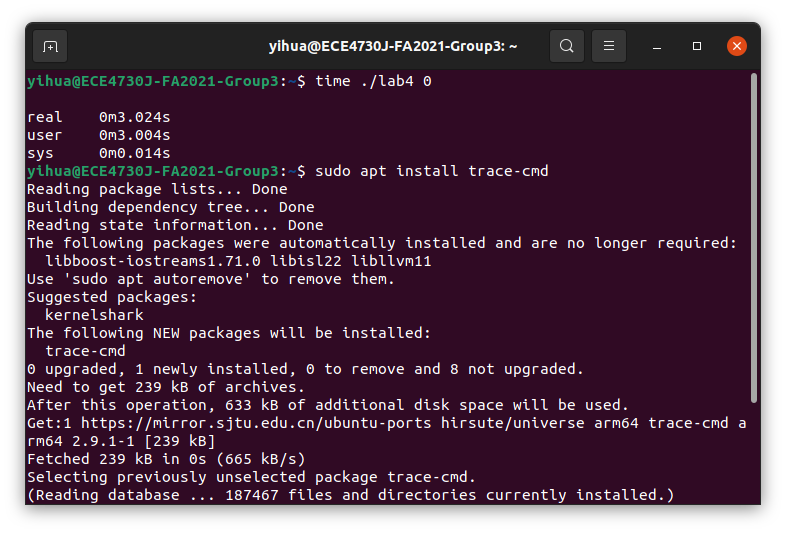
\includegraphics[width=1\textwidth]{1.png}
    \caption{The output from our new program.}
\end{figure}
\noindent2. Please name three processes that interfered with the execution of your program on that core, and explain briefly how you know they did that based on the trace you examined.
\begin{minted}[frame=single,bgcolor=bg,breaklines]{bash}
sudo apt install trace-cmd
sudo trace-cmd record -e sched_switch ./lab3-1 0
sudo apt install kernelshark
kernelshark trace.dat
\end{minted}
\begin{figure}[H]
    \centering
    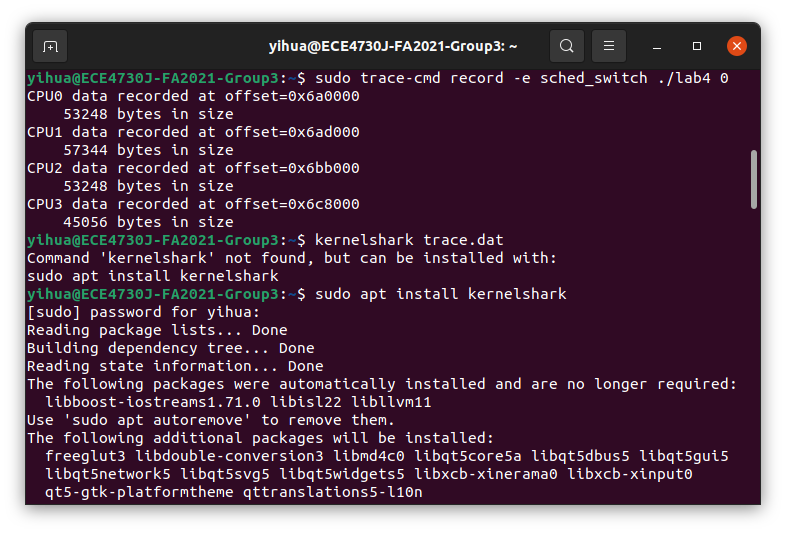
\includegraphics[width=1\textwidth]{2.png}
    \caption{\texttt{trace-cmd original\_track.dat}.}
\end{figure}
\begin{itemize}
    \item \texttt{gnome-system-mo}
    \item \texttt{kworker}
    \item \texttt{v3d\_render}
\end{itemize}
There are also a switch to migration and a switch to swapper in the beginning and in the end.\\
They trigger events \texttt{sched\_switch} from \texttt{lab3-1} to them or from them to \texttt{lab3-1} on the line of CPU 0, so we can know they interfered with the execution of our program on that core (core 0).
\begin{figure}[H]
    \centering
    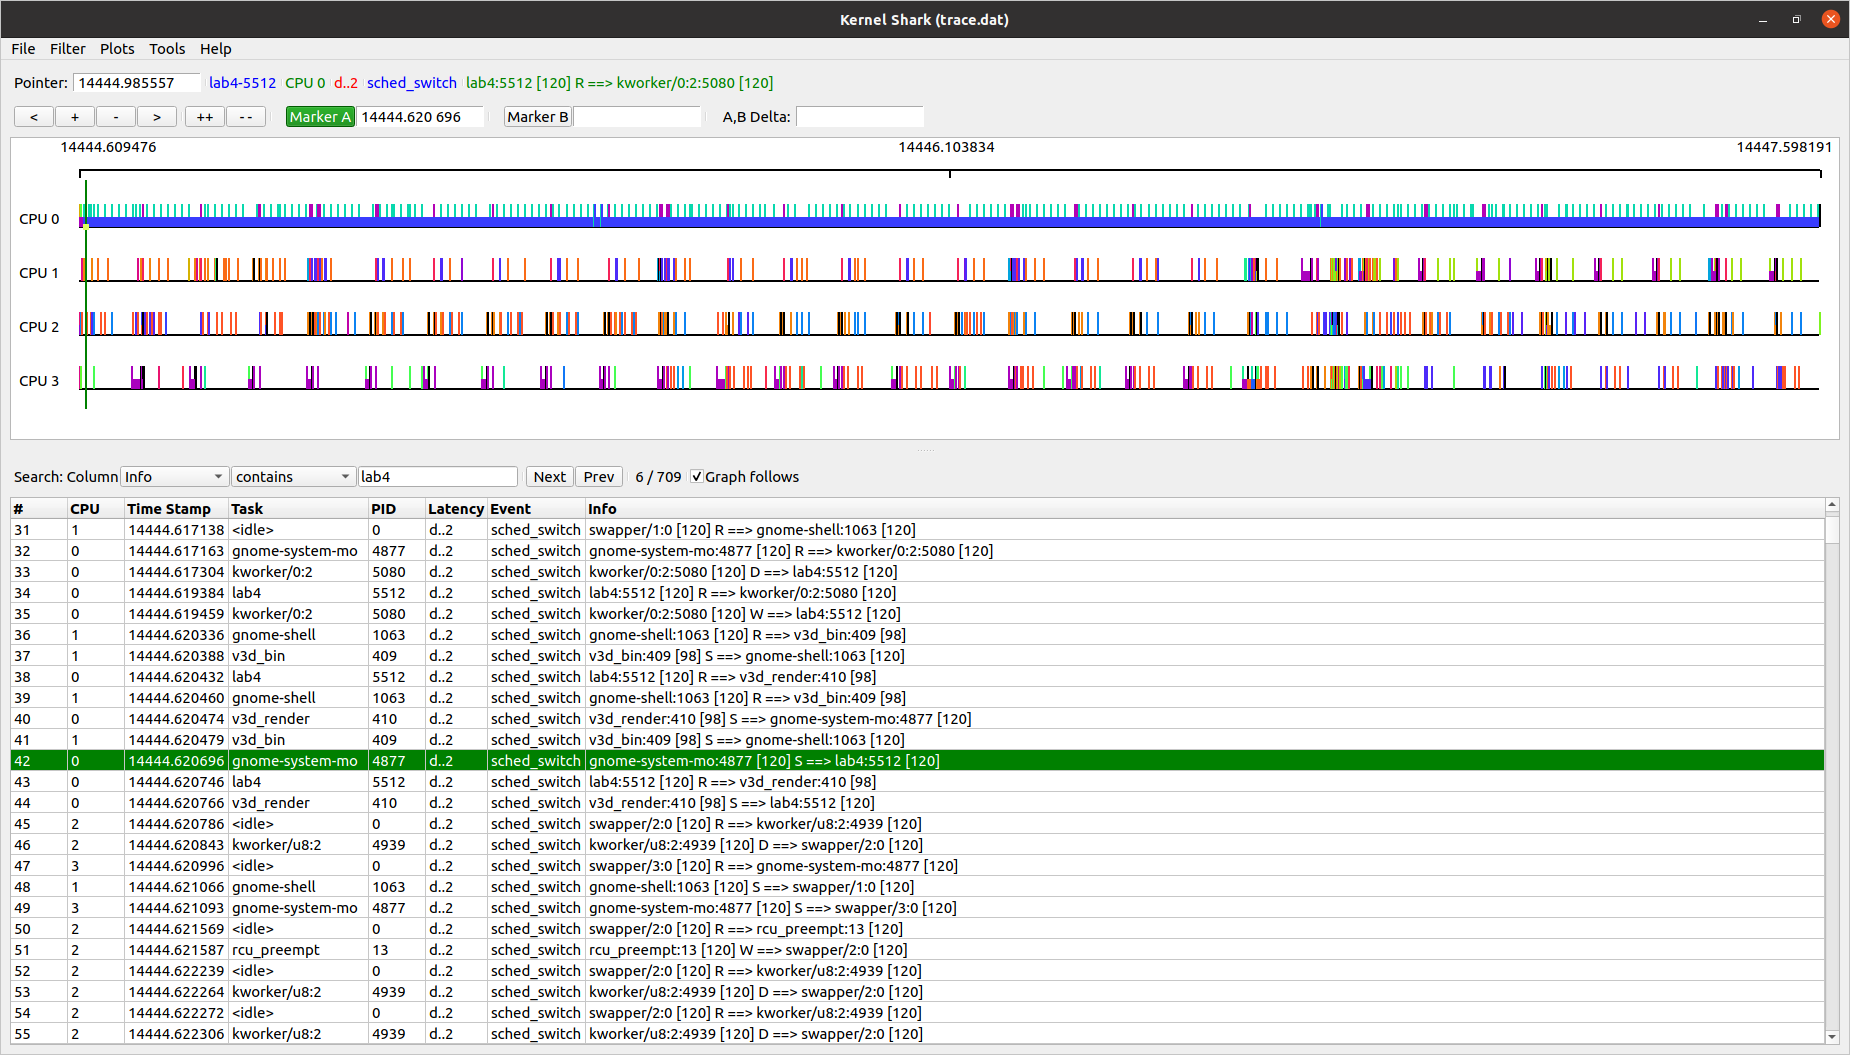
\includegraphics[width=1\textwidth]{3.png}
    \caption{\texttt{kernelshark original\_track.dat}.}
\end{figure}
\noindent3. Find the largest number for which sched\_setscheduler() succeeds when run as root, and the largest number for which sched\_setscheduler() succeeds when run not as root, and report those values as the answer to this exercise.
\inputminted[frame=single,bgcolor=bg,breaklines,linenos]{c}{lab3-2.c}
\begin{figure}[H]
    \centering
    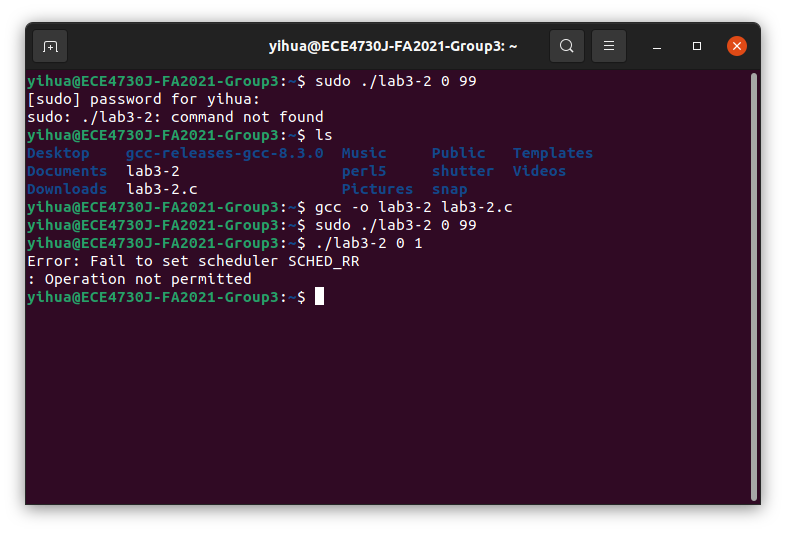
\includegraphics[width=1\textwidth]{4.png}
    \caption{The largest number for which sched\_setscheduler() succeeds when run as root and not as root.}
\end{figure}
The largest number for which sched\_setscheduler() succeeds when run as root is 99. No matter what number is chosen, sched\_setscheduler() never succeeds when run not as root.
\begin{minted}[frame=single,bgcolor=bg,breaklines]{bash}
sudo trace-cmd record -e sched_switch ./lab3-2 0
kernelshark trace.dat
\end{minted}
\begin{figure}[H]
    \centering
    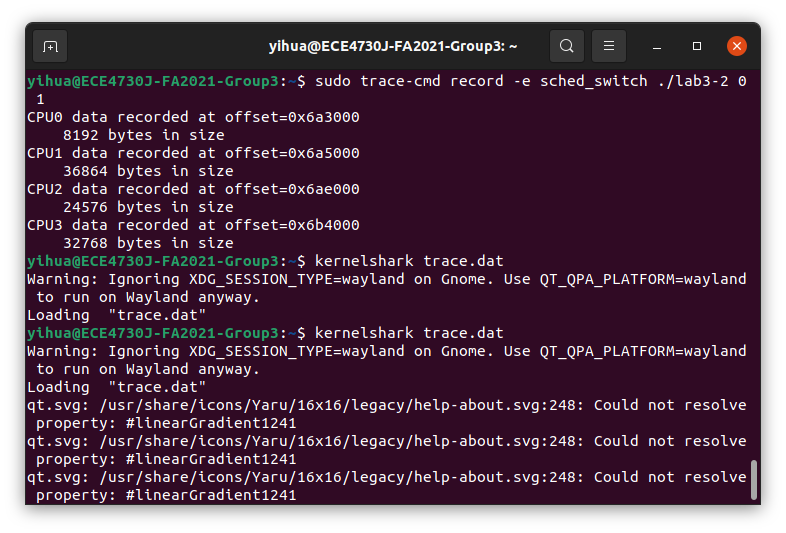
\includegraphics[width=1\textwidth]{5.png}
    \caption{\texttt{kernelshark track.dat}.}
\end{figure}
4. Please state whether any processes preempted your program (and if so which ones), and whether there are any meaningful differences in how these interruptions appear in this trace (kernelshark trace.dat), versus in your original (non-real-time) trace (kernelshark trace\_original.dat).
\begin{figure}[H]
    \centering
    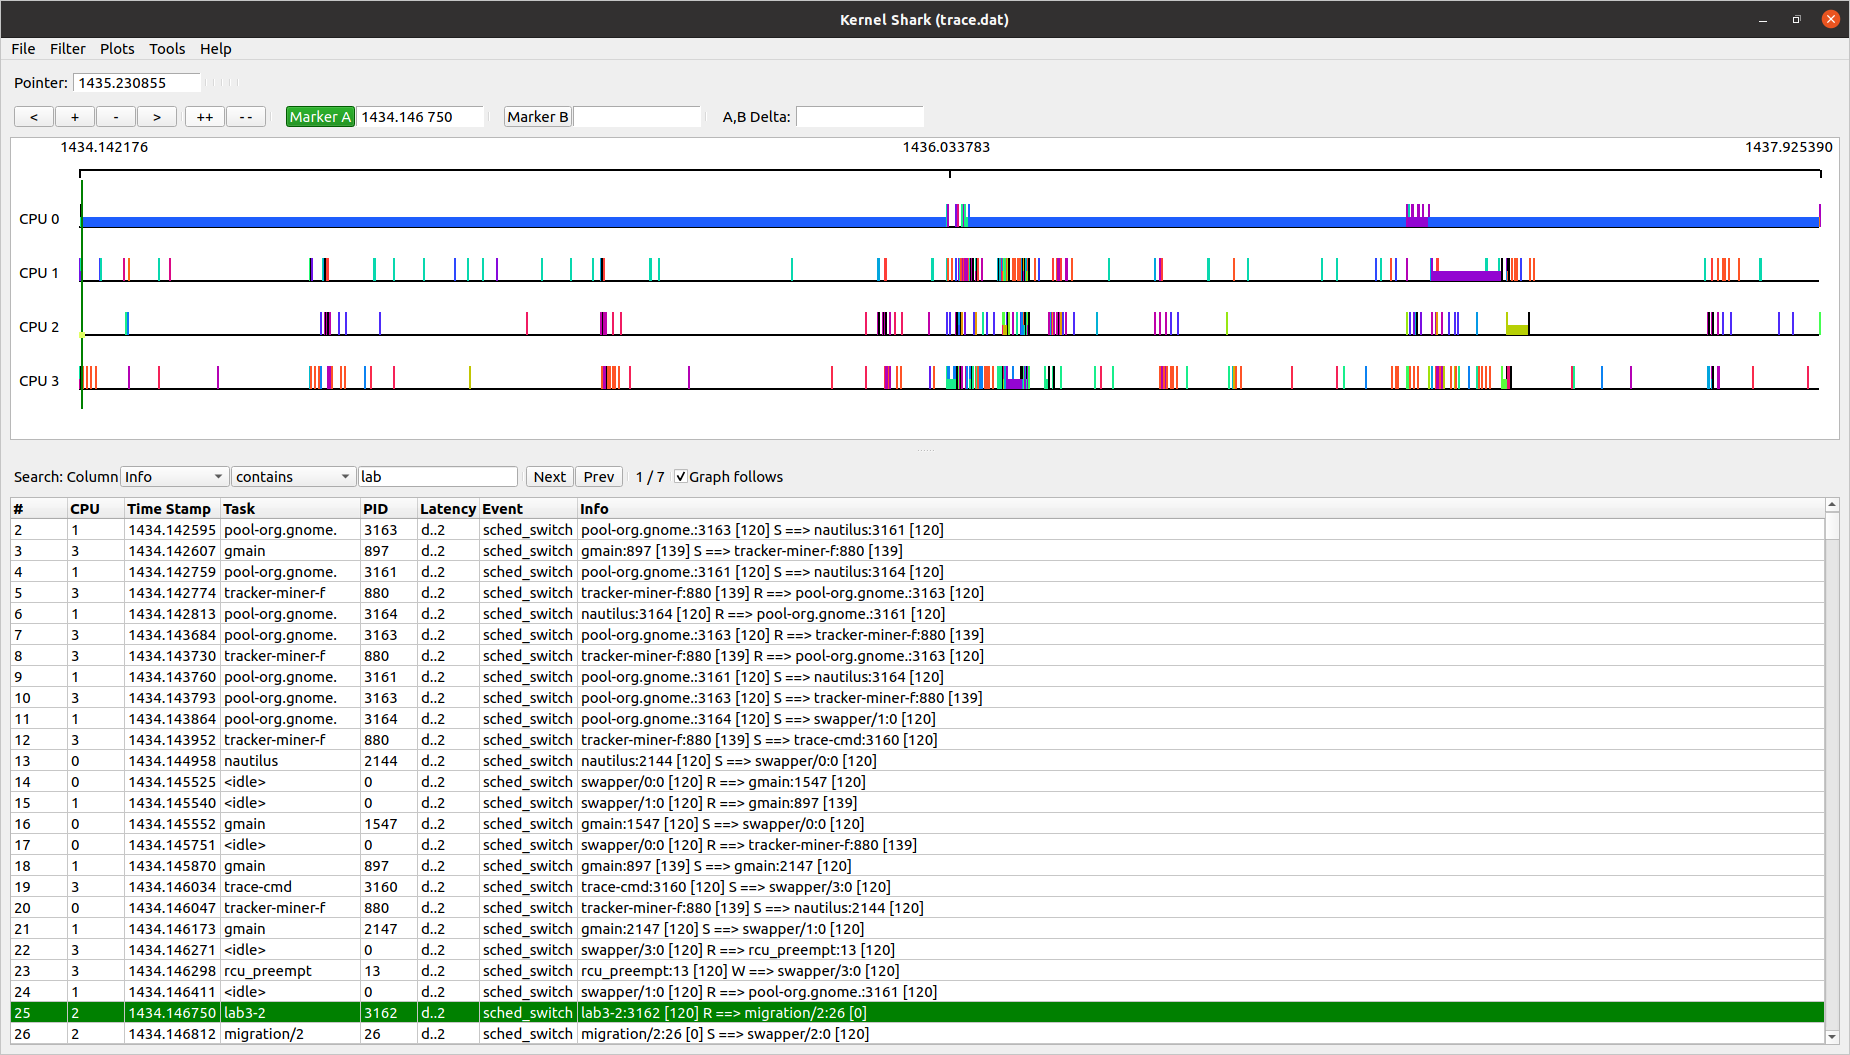
\includegraphics[width=1\textwidth]{6.png}
    \caption{Processes that preempted our program.}
\end{figure}
\begin{itemize}
    \item \texttt{gmain}
    \item \texttt{nautilus}
    \item \texttt{<idle>}
    \item \texttt{tracker-miner-f}
    \item \texttt{ksoftirqd}
    \item \texttt{kworker}
    \item \texttt{brcmf\_wdog/mmc1}
    \item \texttt{migration}
    \item \texttt{tracker-store}
\end{itemize}
Task \texttt{lab3-2} first executed very shortly on CPU 2, then by \texttt{migration->swapper->nautilus} it is switched to CPU 0.

The interruptions of the trace appear much less than the original trace for all the 4 CPUs, especially for CPU 0, there are less sched\_switch in the trace than in the original trace. The price is the execution time of the real-time program is a bit longer than the non-real-time program \cite{mckenney2008real}.

5. Please state how many sched\_switch events were recorded on CPU core 0 where your program ran, and compare that number to the number of sched\_switch events were recorded on each of the other CPU cores.

By using Search:Column, we have the number of sched\_switch events recorded on each CPU:
\begin{table}[H]
    \centering
    \begin{tabular}{|c|c|}
        \hline
        CPU 0&64\\
        \hline
        CPU 1&485\\
        \hline
        CPU 2&314\\
        \hline
        CPU 3&476\\
        \hline
    \end{tabular}
    \caption{The number of sched\_switch events recorded on each CPU.}
\end{table}
The number of sched\_switch events recorded on CPU 1, 2, and 3 are much more than those on CPU 0.

6. Please state (1) what range of real-time priorities you see being used, (2) what processes have real-time priorities, and (3) speculate why they may need to be run with real-time priority.
\begin{figure}[H]
    \centering
    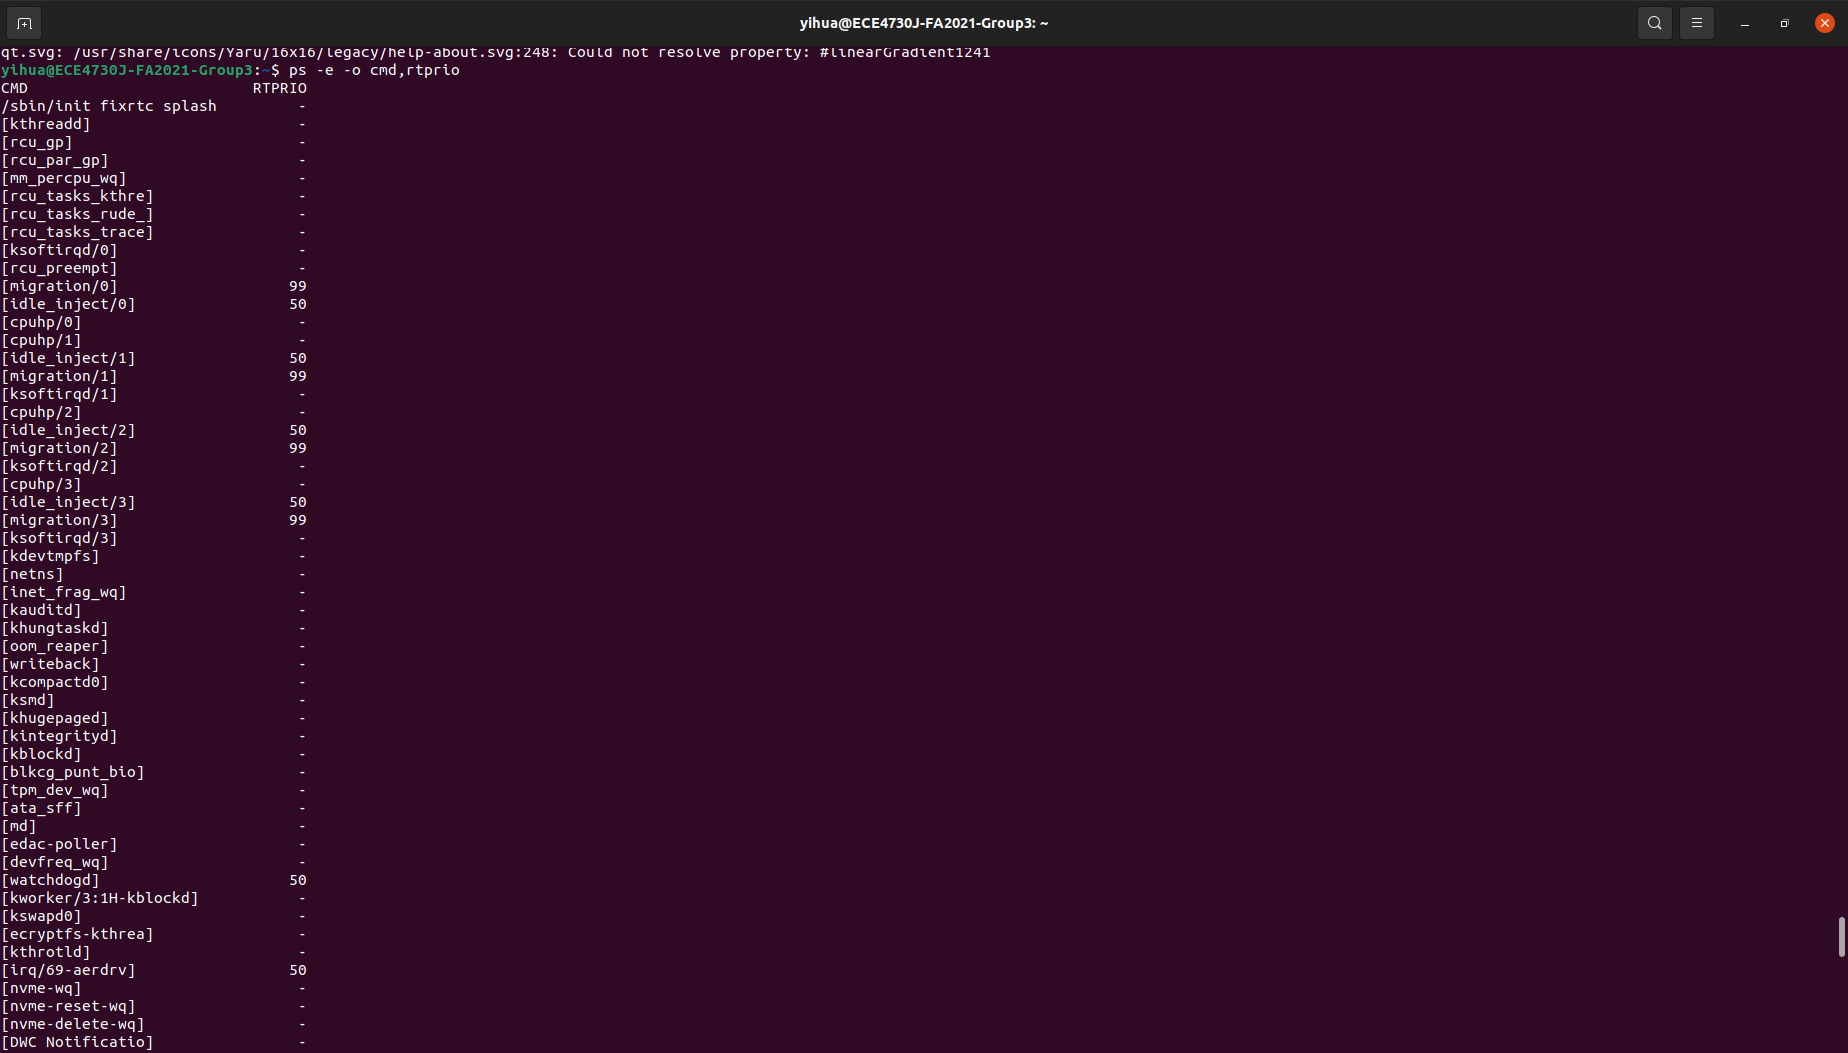
\includegraphics[width=1\textwidth]{7.png}
    \caption{Real-time priorities.}
\end{figure}
(1) They use real-time priorities ranging from 0 to 99 (but only values of 0, 1, 50, 99 are used).

(2)
\begin{table}[H]
    \centering
    \begin{tabular}{|c|c|}
        \hline
        [migration/0]&99\\
        \hline
        [idle\_inject/0]&50\\
        \hline
        [idle\_inject/1]&50\\
        \hline
        [migration/1]&99\\
        \hline
        [idle\_inject/2]&50\\
        \hline
        [migration/2]&99\\
        \hline
        [idle\_inject/3]&50\\
        \hline
        [migration/3]&99\\
        \hline
        [watchdogd]&50\\
        \hline
        [irq/69-aerdrv]&50\\
        \hline
        [irq/55-mmc0]&50\\
        \hline
        [v3d\_bin]&1\\
        \hline
        [v3d\_render]&1\\
        \hline
        [v3d\_tfu]&1\\
        \hline
        [v3d\_csd]&1\\
        \hline
        [v3d\_cache\_clean]&1\\
        \hline
        [irq/46-vc4 hdmi]&50\\
        \hline
        [irq/47-vc4 hdmi]&50\\
        \hline
        [irq/43-vc4 hdmi]&50\\
        \hline
        [irq/42-vc4 hdmi]&50\\
        \hline
        [irq/52-vc4 hdmi]&50\\
        \hline
        [irq/53-vc4 hdmi]&50\\
        \hline
        [irq/49-vc4 hdmi]&50\\
        \hline
        [irq/48-vc4 hdmi]&50\\
        \hline
        [card1-crtc0]&50\\
        \hline
        [card1-crtc1]&50\\
        \hline
        [card1-crtc2]&50\\
        \hline
        [card1-crtc3]&50\\
        \hline
        [card1-crtc4]&50\\
        \hline
        [card1-crtc5]&50\\
        \hline
        /usr/libexec/tracker-miner-&0\\
        \hline
    \end{tabular}
    \caption{Processes that have real-time priorities.}
\end{table}
(3) They may need to be run with real-time priority because they are related to irq (interrupt requests), system idle, watchdog, migration, HDMI, or card. Some of them are related to drivers. System must schedule these CMDs real-time to run normally.

7. Please state (1) how many sched\_switch events occur on your program's processor, (2) whether your program is ever preempted, and if so (3) when and where is it preempted?
\begin{figure}[H]
    \centering
    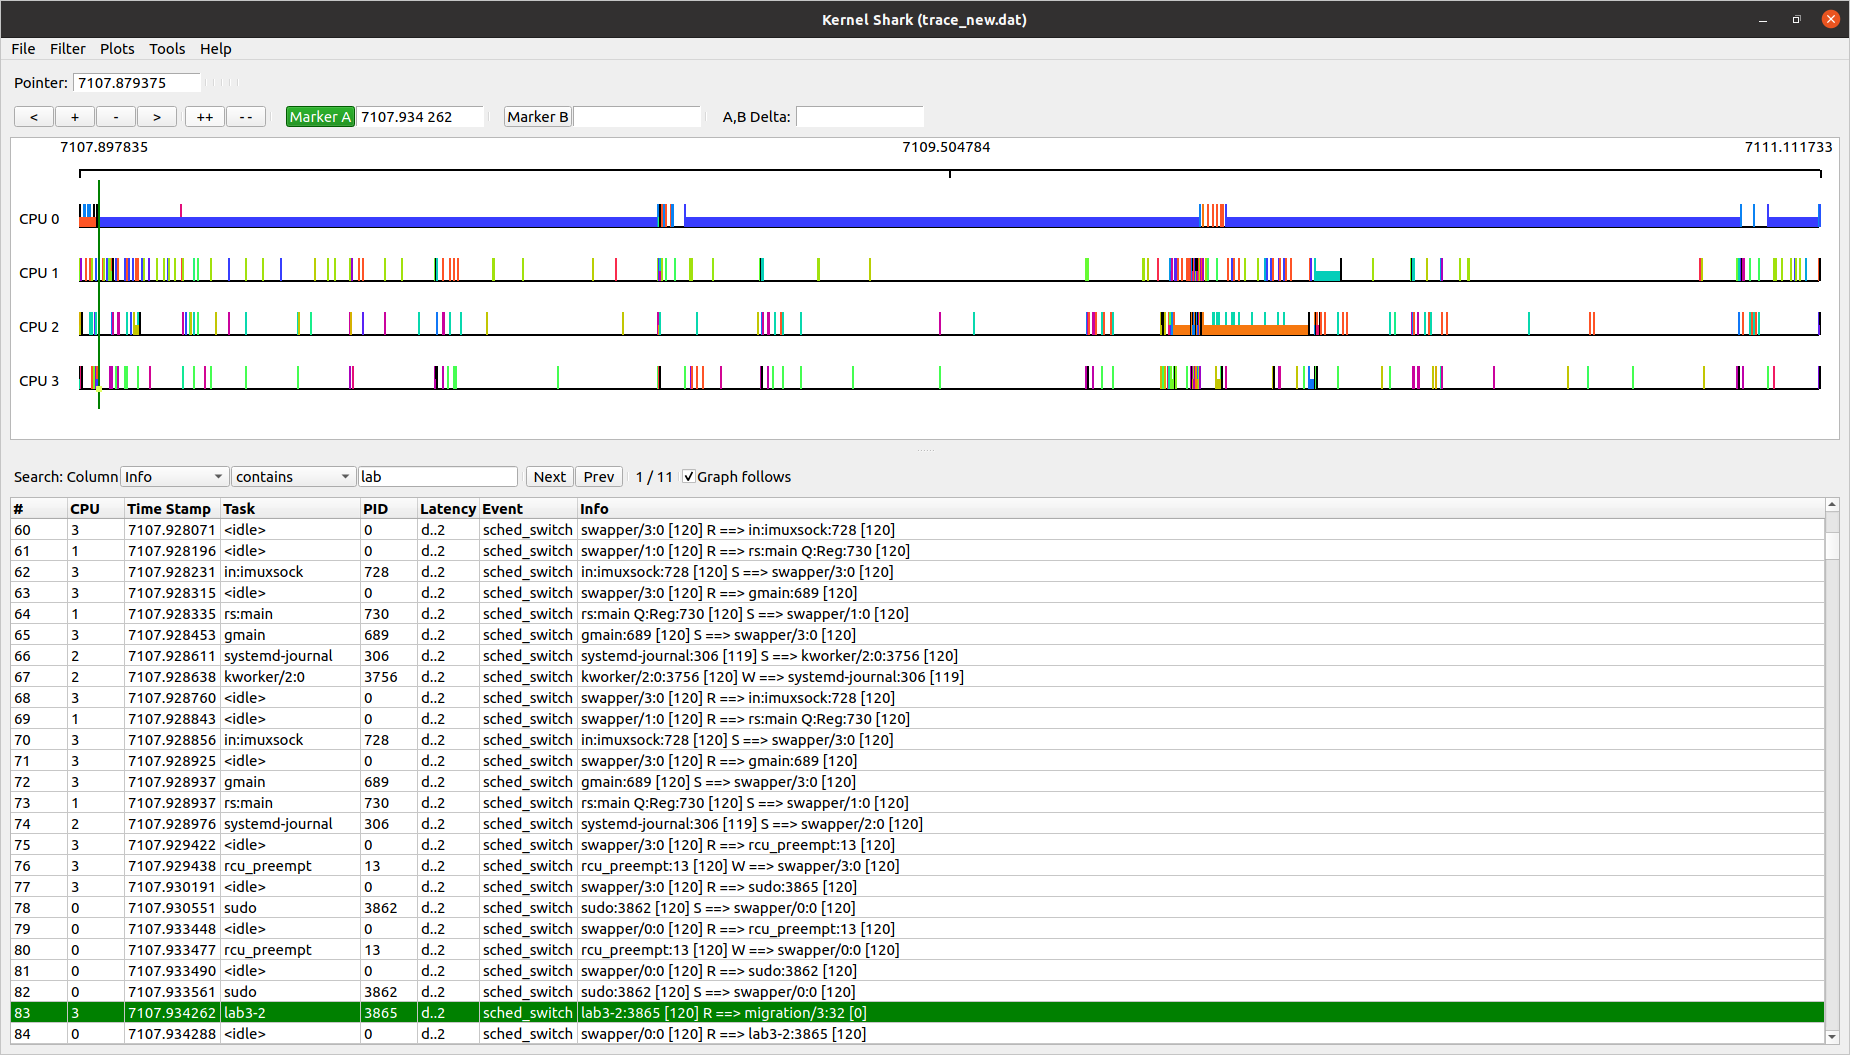
\includegraphics[width=1\textwidth]{8.png}
    \caption{\texttt{kernelshark new\_track.dat}.}
\end{figure}
(1) 117 sched\_switch events occur on your program's processor (CPU 0).

(2) Our program is preempted.

(3) It is preempted at \texttt{tracker-miner-f, <idle>, nautilus, kworker, rcu\_preempt, gdbus, trace-cmd, pool-tracker-st, ksoftirqd}.
\printbibliography
\end{document}